\subsection{Métodos}\label{sec:methods}
Esta pesquisa adota uma abordagem descritiva-experimental, cujo objetivo é avaliar a viabilidade de implementação do sistema de informação ESPEON para eventual avaliação pedagógica. A coleta de dados será feita sob turmas de diferentes áreas do conhecimento, a fim de garantir maior representatividade e diversidade no conjunto de dados.

O experimento será conduzido com a participação voluntária de alunos matriculados em três disciplinas distintas, no contexto do ensino superior; com amostragem não probabilística, por conveniência. Os dados serão coletados a partir dos \textit{logs} de navegação gerados pela extensão, incluindo eventos como mudanças de aba, minimização da janela da conferência, e o uso de periféricos como microfone e câmera.

Os indicadores extraídos serão armazenados em um banco de dados não relacional, MongoDB, e processados no \textit{backend} Python da aplicação, para posteriormente gerar relatórios de desempenho em formato PDF. Abaixo, a Figura \ref{fig:arquiteturaLogs} ilustra o processo de captura e armazenamento dos logs, enquanto a Figura \ref{fig:arquiteturaReports} ilustra a arquitetura procedural para emnissão dos relatórios.

\begin{figure}[ht]
    \centering
    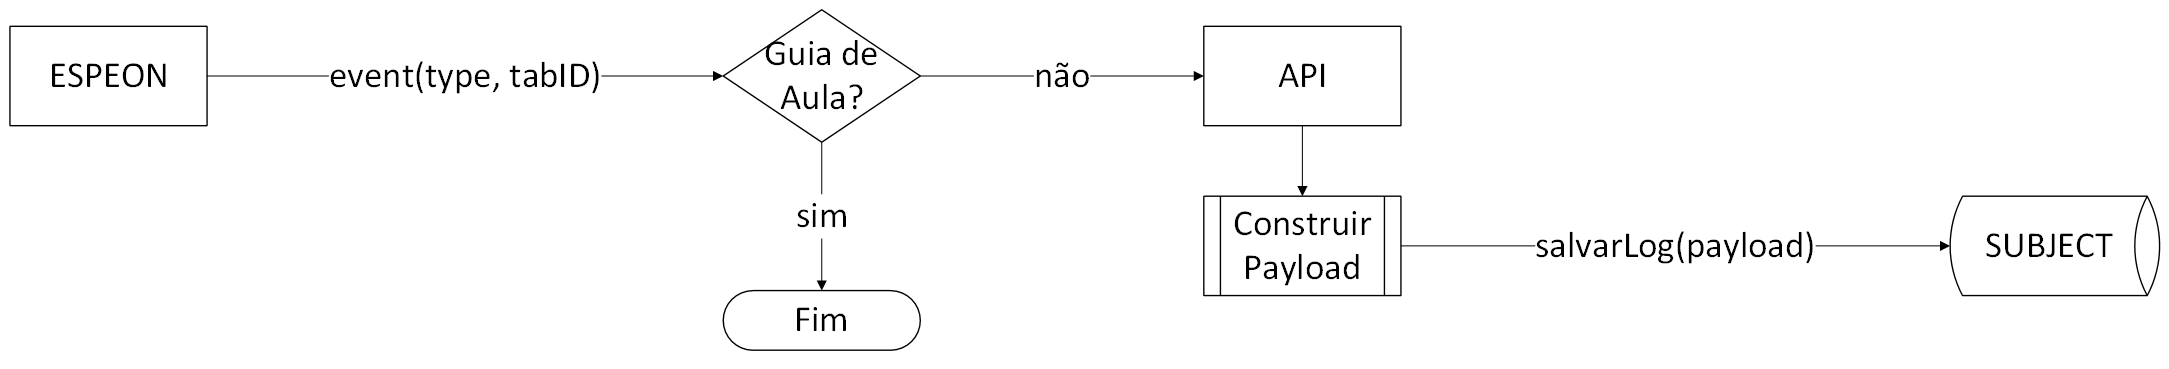
\includegraphics[width=.97\textwidth]{assets/images/arquitetura.logs.png}
    \caption{Arquiterua Procedural: Logs}
    \label{fig:arquiteturaLogs}
\end{figure}

\begin{figure}[ht]
    \centering
    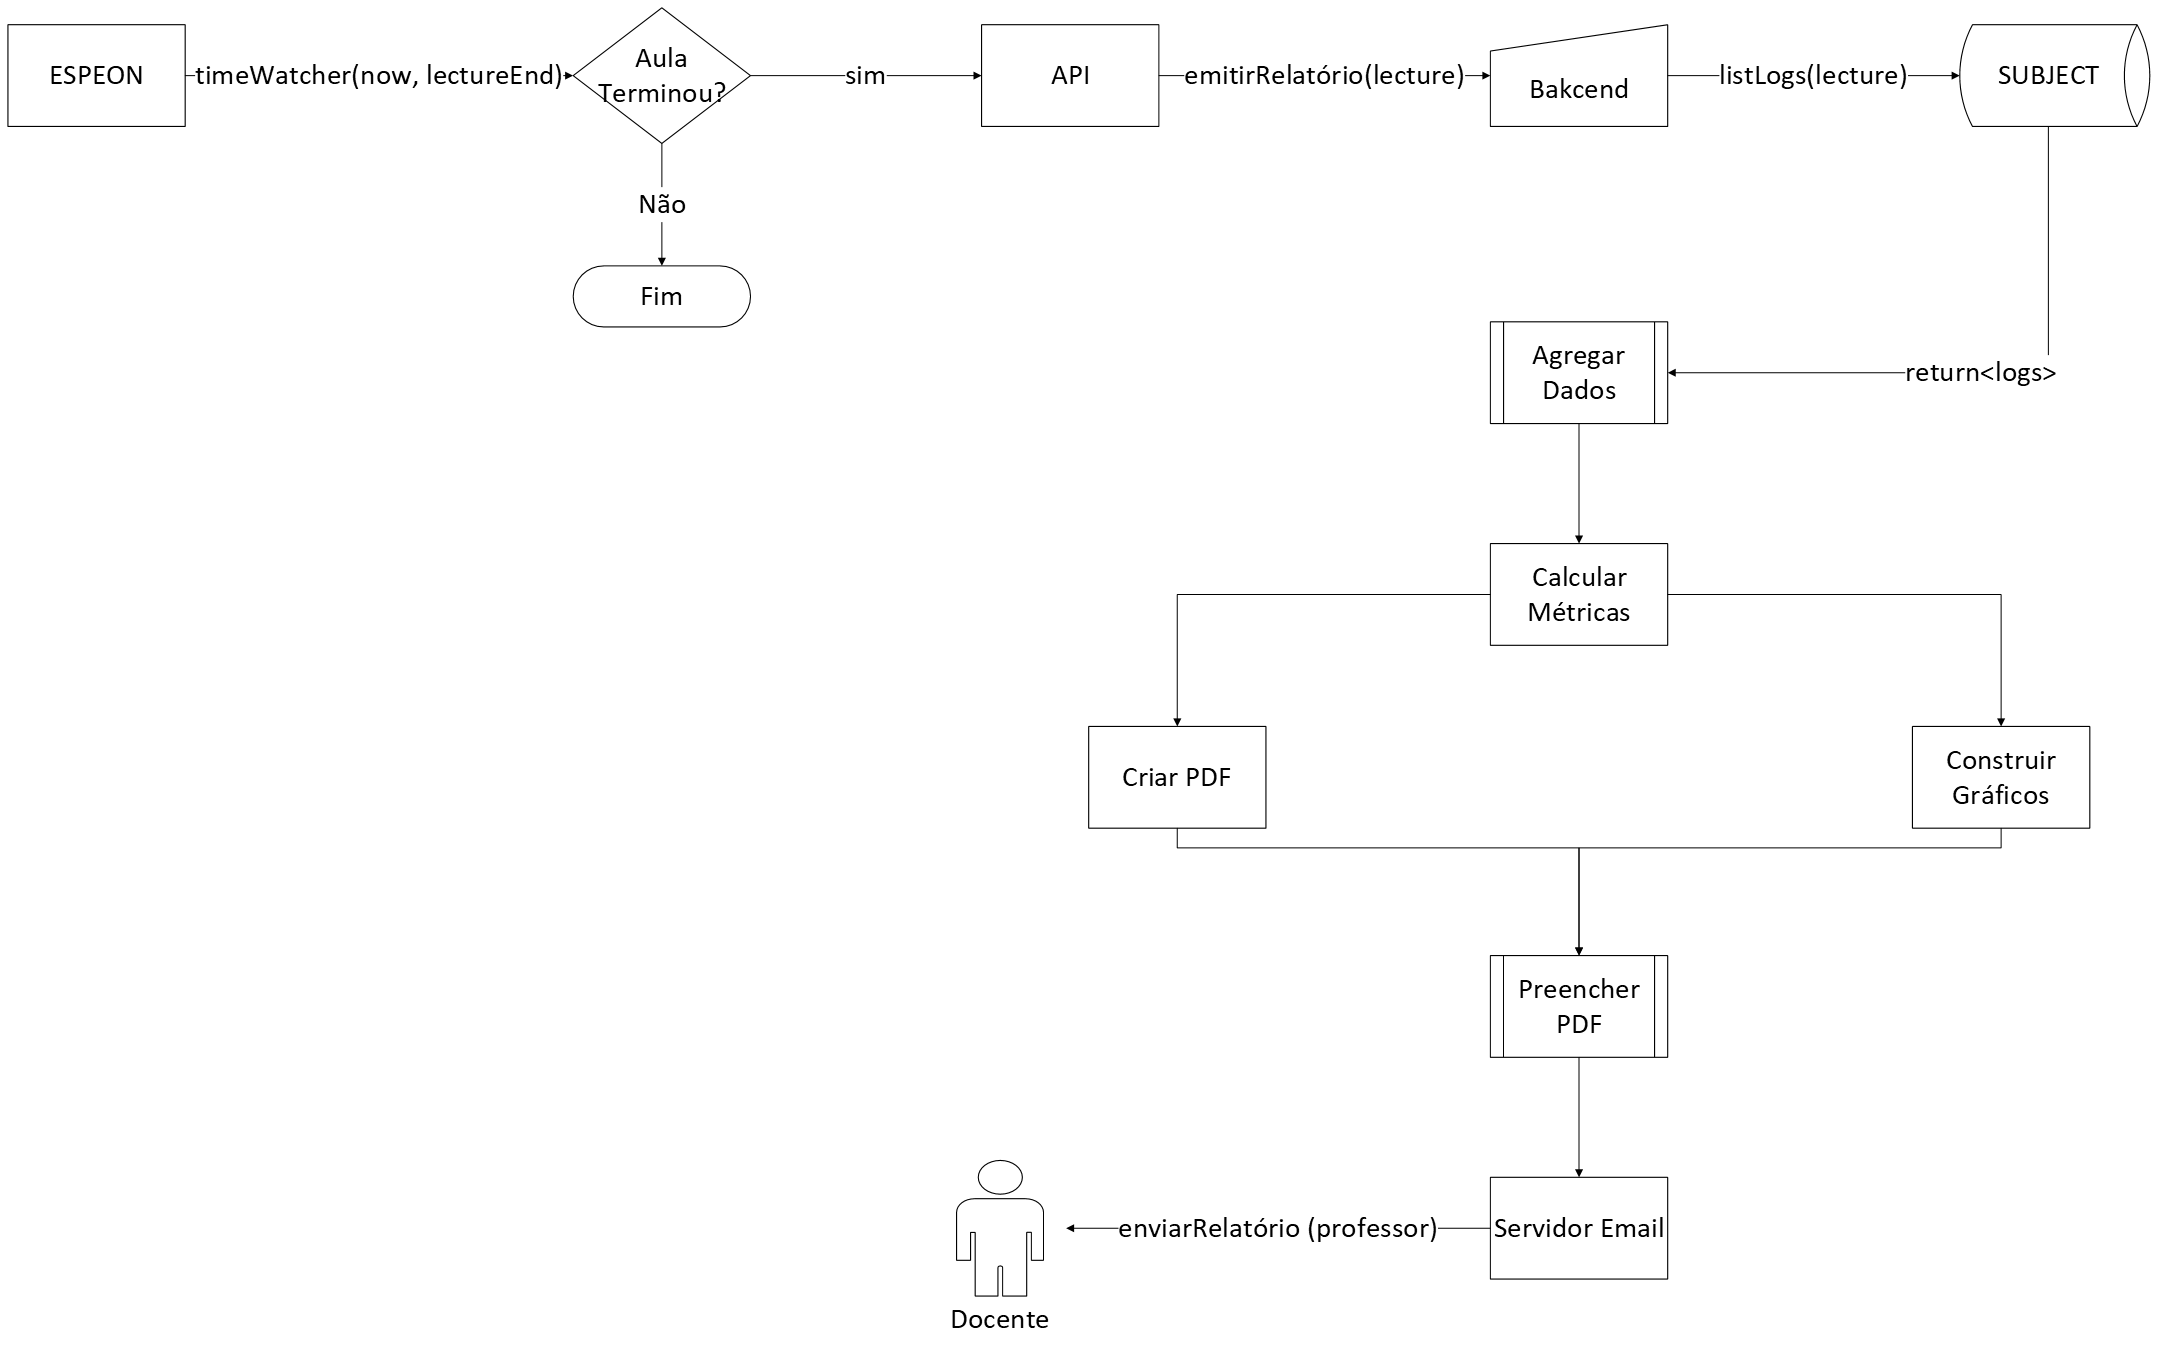
\includegraphics[width=.97\textwidth]{assets/images/arquitetura.reports.png}
    \caption{Arquiterua Procedural: Relatórios}
    \label{fig:arquiteturaReports}
\end{figure}

A análise dos dados será realizada por meio de estatísticas descritivas — como média, desvio padrão e frequências —  com o objetivo de identificar padrões de comportamento entre os grupos analisados. A comparação entre disciplinas permitirá avaliar o impacto da área do conhecimento sobre os níveis de atenção e engajamento dos estudantes. Uma versão experimental dos relatórios pode ser observada na Figura \ref{fig:report} a seguir.

\begin{figure}[ht]
    \centering
    \includegraphics[width=.99\textwidth]{assets/images/relatório.png}
    \caption{Relatório de Disciplina}
    \label{fig:report}
\end{figure}

Como indicadores de atenção, foram agrupadas as guias, que não a correspondente à aula; ilustrando os sites mais acessados pelos alunos durante a aula. Já como indicativos de engajemento, há análise das permissões dadas aos periféricos de áudio e vídeo, bem como o \textit{streaming} de dados por eles feito.


Todos os participantes serão informados previamente sobre os objetivos do estudo, e o uso dos dados seguirá as diretrizes éticas da pesquisa com seres humanos, com ênfase na privacidade e na conformidade com a Lei Geral de Proteção de Dados (LGPD).
